\section{Introduction}
The Microsoft Intune family of products is an integrated solution for managing all of your devices.

The following Microsoft management solutions are all now part of the Microsoft Intune brand:
\begin{itemize}
    \item 
        Configuration Manager
    \item
        Intune
    \item
        Endpoint analytics
    \item
        Autopilot
\end{itemize}

the Configuration Manager console to configure sites and clients, and to run and monitor management tasks. This console is the main point of administration, and lets you manage multiple sites.

You can install the Configuration Manager console on additional computers, and restrict access and limit what administrative users can see in the console by using Configuration Manager role-based administration.

usage:
\begin{itemize}
    \item inventory management
    \item software deployment
    \item software updates management
    \item OS deployment
    \item compliance management
    \item reporting
\end{itemize}


\subsection{sites and hierarchies}
A Configuration Manager deployment must be installed in an Active Directory domain. The foundation of this deployment includes one or more Configuration Manager sites that form a hierarchy of sites. From a single site to a multi-site hierarchy, the type and location of sites you install provide the ability to scale up (expand) your deployment when necessary, and deliver key services to managed users and devices.

When you install Configuration Manager for the first time, the first Configuration Manager site that you install determines the scope of your hierarchy. The first Configuration Manager site is the foundation from which you will manage devices and users in your enterprise. This first site must be: 
\begin{itemize}
    \item 
        either a {\bf central administration site (CAS)}: allows to manage all the primary sites from one point, make some reporting, and is totally optional. CAS does not directly support management of devices. CAS needs one or more \href{https://learn.microsoft.com/en-us/mem/configmgr/core/plan-design/hierarchy/design-a-hierarchy-of-sites#BKMK_ChoosePriimary}{primary sites} as child sites which are in charge to manage devices.
    \item 
        or a stand-alone primary site
\end{itemize}

A \href{https://learn.microsoft.com/en-us/mem/configmgr/core/plan-design/hierarchy/design-a-hierarchy-of-sites#BKMK_ChooseSecondary}{secondary site} can only be installed as a child site below a primary site. This site type extends the reach of a primary site to manage devices in locations that have a slow network connection to the primary site. Even though a secondary site extends the primary site, {\bf the primary site manages all of the clients}.

In case of high availability in required, it is also possible to find a passive site server that will be used only if the active site server stop working

\subsection{site system servers and site system roles}


\begin{figure}[!ht]
  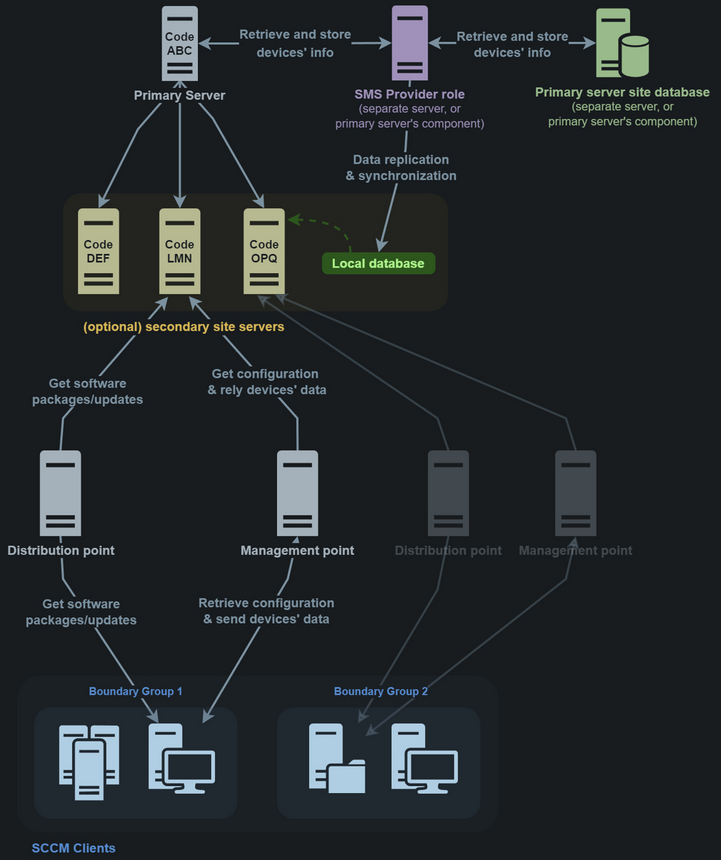
\includegraphics[width=\linewidth]{network/mecm/images/archi.png}
  \caption{Archi MECM}
  \label{fig:mecm-archi}
\end{figure}



Each Configuration Manager site includes a site server that's a {\bf site system server}. The site can also include additional site system servers on computers that are remote from the site server. Site system servers (the site server or a remote site system server) support site system roles.

Different Configuration Manager sites (CAS, primary, secondary) can support different sets of site system roles. The supported set of site system roles depends on the type of site. For example, the service connection point is only supported at the top-tier site of the hierarchy. The top-tier site might be a central administration site or a standalone primary site. This role isn't supported at a child primary site or at secondary sites.

\subsubsection{Site database server}
The site assigns \href{https://learn.microsoft.com/en-us/mem/configmgr/core/plan-design/hierarchy/plan-for-the-site-database}{this role} to site system servers that hold an instance of the site database. This database is used by the site server to retrieve and store information about the managed devices and is also used by the management point to retrieve policies and configuration information needed by the SCCM clients.


\subsubsection{Systems Management Server (SMS)}

The \href{https://learn.microsoft.com/en-us/mem/configmgr/core/plan-design/hierarchy/plan-for-the-sms-provider#about}{SMS Provider} is a Windows Management Instrumentation (WMI) provider that assigns read and write access to the Configuration Manager database at a site.


\subsubsection{Management point}

A site system role that provides policy and service location information (configuration to communicate with the site server) to clients. It also receives configuration data from clients.

Primary sites support multiple instances of this role. Secondary sites support a single management point.

To help reduce the processing load placed on the site database server by management points as they service requests from clients, use Database replicas for management points.

\subsubsection{Distribution point}

A site system role that contains source files for clients to download, for example:
\begin{itemize}
    \item 
        Application content
    \item
        Software packages
    \item
        Software updates
    \item
        OS images
    \item
        Boot images
\end{itemize}

By default, this role installs on the site server when you install a new primary or secondary site. This role isn't supported at a central administration site.

\subsubsection{Software update point}
A site system role that integrates with Windows Server Update Services (WSUS) to provide software updates to Configuration Manager clients

\subsubsection{Other elements}
\begin{itemize}
    \item Asset Intelligence synchronization point
    \item Certificate registration point
    \item Cloud management gateway connection point
    \item Endpoint Protection point
    \item Enrollment point
    \item State migration point (stores user state data during  migration ofa computer to a new operating system)
    \item \ldots
\end{itemize}

\subsection{Boundary / Boundary group}

\href{https://learn.microsoft.com/en-us/mem/configmgr/core/servers/deploy/configure/boundaries}{Boundaries} are locations (AD site, IP range, IP subnet\ldots) on the network that contains devices to manage. boundaries can be created manually or using \href{https://learn.microsoft.com/en-us/mem/configmgr/core/servers/deploy/configure/about-discovery-methods#bkmk_aboutForest}{Active Directory forest discovery}

\href{https://learn.microsoft.com/en-us/mem/configmgr/core/servers/deploy/configure/boundary-groups}{Boundary groups}  organize boundaries. Clients use a boundary group for:
\begin{itemize}
    \item \href{https://learn.microsoft.com/en-us/mem/configmgr/core/clients/deploy/assign-clients-to-a-site#automatic-site-assignment}{Automatic site assignment}
    \item To find a site system server that can provide a service, including:
    \begin{itemize}
        \item \href{https://learn.microsoft.com/en-us/mem/configmgr/core/plan-design/hierarchy/plan-for-site-system-servers-and-site-system-roles#distribution-point}{Distribution points} for content location.
        \item \href{https://learn.microsoft.com/en-us/mem/configmgr/core/plan-design/hierarchy/plan-for-site-system-servers-and-site-system-roles#software-update-point}{Software update points}
        \item State migration points
        \item \href{https://learn.microsoft.com/en-us/mem/configmgr/core/plan-design/hierarchy/plan-for-site-system-servers-and-site-system-roles#management-point}{Management points}
        \item Preferred management points
        \item Cloud management gateway (CMG) for policy and content
    \end{itemize}
\end{itemize}

\subsection{Client agent}

When SCCM is installed in an Active Directory, the clients can be deployed on the workstations by six different ways:
\begin{itemize}
    \item 
        Client push installation (default)
    \item
        Software update-based installation
    \item
        Group Policy installation
    \item
        Manual installation
    \item
        Logon script installation
    \item
        Package and program installation
\end{itemize}

The first way of deploying SCCM is the Client push installation method, which is the default one and the least secure.

This installation will use "client push accounts". They are service accounts with local administrative rights on the assets where SCCM will have to deploy some stuff. The system administrator creates groups of endpoints and for each of those, one "client push account". For each group, only one "client push account" can authenticate with administrator rights on the assets of this group. Thus, if an account is compromised, only the members of the corresponding group can be compromised in turn.

When the SCCM deployment is launched, it will basically try to authenticate with each client push accounts on each asset, and if the authentication fails, SCCM will try the next account in line. When the authentication succeeds, it moves to the following asset, and so on until the deployment is complete.

SCCM deployment via Client push installation is service accounts credentials spraying in a nutshell.

Nota bene, there is a feature allowing for \href{https://learn.microsoft.com/en-us/mem/configmgr/core/clients/deploy/deploy-clients-to-windows-computers#configure-the-site-to-automatically-use-client-push-for-discovered-computers}{automatic client push installation} on all discovered clients in a boundary group in an SCCM site.

